\documentclass{article}
\usepackage{geometry}
\usepackage{fancyhdr}
\usepackage{amsmath, amsthm, amssymb}
\usepackage{graphicx}
\usepackage{hyperref}
\usepackage{color}
\usepackage{listings}
\lstset{ %
language=C++,                % choose the language of the code
basicstyle=\footnotesize,       % the size of the fonts that are used for the code
numbers=left,                   % where to put the line-numbers
numberstyle=\footnotesize,      % the size of the fonts that are used for the line-numbers
stepnumber=1,                   % the step between two line-numbers. If it is 1 each line will be numbered
numbersep=5pt,                  % how far the line-numbers are from the code
backgroundcolor=\color{white},  % choose the background color. You must add \usepackage{color}
showspaces=false,               % show spaces adding particular underscores
showstringspaces=false,         % underline spaces within strings
showtabs=false,                 % show tabs within strings adding particular underscores
frame=single,           % adds a frame around the code
tabsize=2,          % sets default tabsize to 2 spaces
captionpos=b,           % sets the caption-position to bottom
breaklines=true,        % sets automatic line breaking
breakatwhitespace=false,    % sets if automatic breaks should only happen at whitespace
escapeinside={\%*}{*)}          % if you want to add a comment within your code
}
\begin{document}

\title{Cryptographic Analysis}
\author{Colin Rice}
\author{Samuel Milito}
\author{Jacob Shedd}

\maketitle


\section{Race Conditions}

The code as-is provides no protections on money, i.e., there are no mutex locks. For example, the withdrawl function:
\begin{lstlisting}
bool processWithdraw (std::vector<std::string> info)
{
	float b = (float)atof(info.at(4).c_str());
	if(b > 1000.00) {
		return false;
	}

	std::vector<Account>::iterator it;
	for (it = Database.begin(); it != Database.end(); it++) {
====>	if(it->get_un() == info.at(1) && it->get_logged_in() && b <= it->get_balance() && it->get_withdraw() + b <= 1000.00) {
			it->reduce_balance(b);
			it->increase_withdraw (b);
			return true;
		}
	}
	return false;
}
\end{lstlisting}
That is, a user logged on multiple times could theoretically withdraw double the amount in their account, assuming that the timing went through correctly. They would need to pass the marked line at the same time on two consoles, and it will authorize withdrawal on two ATMs, regardless if it would go over the account balance or the daily \$1000 limit. The only protection against this is not allowing users to log in on multiple machines at a time. However, the login function is also succeptible to a race condition:
\begin{lstlisting}
bool login (std::vector<std::string> info) 
{
	std::vector<Account>::iterator it;
	int pin = atoi(info.at(3).c_str());

	for (it = Database.begin(); it != Database.end(); it++) {
===>	if(it->get_un() == info.at(1) && it->get_pin() == pin && !it->get_logged_in() && !it->get_locked()) {
			it->set_logged_in_true ();
			return true;
		} 
		else if(it->get_un() == info.at(1) && it->get_pin() != pin && !it->get_logged_in()) {
			it->increase_login_attempts();
			if(it->get_login_attempts() >= 3) {
				it->lock();
			}
			return false;
		}
	}
	return false;
}
\end{lstlisting}
If the timing works out correctly, a user will pass all required checks (the highlighted line), and then set\_logged\_in\_true will be called. During this time, any other ATMs can then theoretically pass the same checks. The end result is that a single user would be logged on at multiple ATMs. Due to how fast all of the operations are (the data sets are miniscule), a demonstration was not feasible. This issue is exacerbated by the thirty second timeout window for packets (i.e., the bank accepts a packet if it's no more than 30 seconds old), as the proxy could hold packets, making sure that they are sent to the bank at identical times.

With a user logged on to multiple ATMs, they can abuse the race conditions to withdraw or transfer double their account balance.

\section{Invalid Transfers}
A transfer to an invalid user succeeds initially, as the checks are done out of order, namely the highlighted lines:
\begin{lstlisting}
bool processTransfer (std::vector<std::string> info)
{
	float b = (float)atof(info.at(4).c_str());
	if(b > 1000.00) {
		return false;
	}

	std::vector<Account>::iterator it;
	for (it = Database.begin(); it != Database.end(); it++) {
		if(it->get_un() == info.at(1) && it->get_logged_in() && b <= it->get_balance() && it->get_transfer() + b <= 1000.00) {
===>		it->reduce_balance(b);
===>		it->increase_transfer (b);
			std::vector<Account>::iterator foo;
			for (foo = Database.begin(); foo != Database.end(); foo++) {
				if(foo->get_un() == info.at(5) && foo->get_balance() + b <= MAX_BAL) {
					foo->increase_balance (b);
					return true;
				}
			}
		}
	}
	return false;
}
\end{lstlisting}
The active user has their account debited before the targetted user has their account credited. The result is that issuing a transfer to an invalid user will result in the active ATM user losing money, which then vanishes entirely from the system. In the image, Bob has \$40 vanish when he attempts to transfer it to Vriska, a nonexistant user.
\\
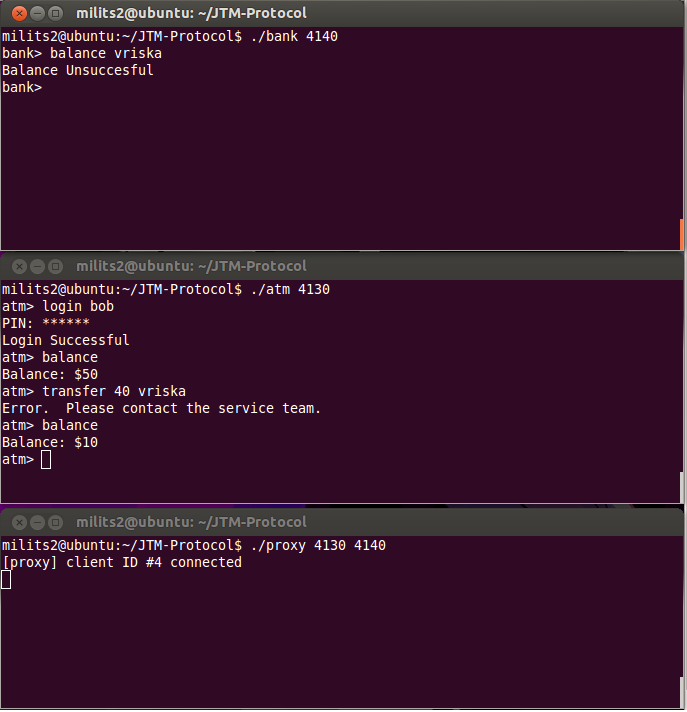
\includegraphics[scale=0.5]{transferLoss.png}
\\

\section{Overly Generous Timeouts}
The timeout checking on both sides is overly generous. The ATM has a 30 second window
\begin{lstlisting}
if(time(NULL) - messageTimeout < 30) // Bank Response needs to be in less that 30 seconds.
{
    // [...]
}
\end{lstlisting}
and the bank has no timeout handling at all. As such, packets can be held up to 30 seconds before being sent to the ATM, and indefinitely before being sent to the bank. This opens it up to much longer analysis than otherwise. While there is no specific exploit I have in mind, this is a much larger window than is needed for packets to be sent and received. In the proxy, a large amount of work can be done. Adding the following code in between receiving an ATM packet and forwarding the packet to the bank results in proper operation:
\begin{lstlisting}
printf( "Sleeping for 29 seconds.\n" );
sleep( 29 );
\end{lstlisting}
An example is below.
\\
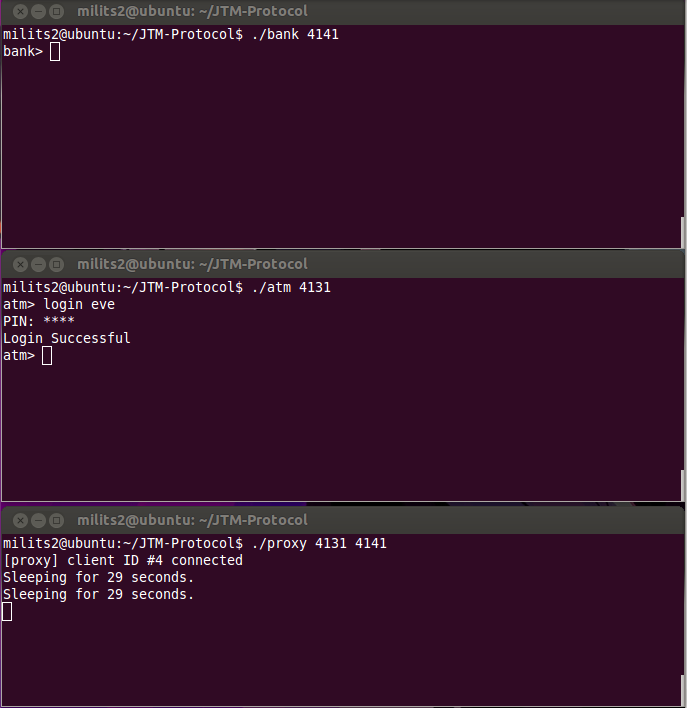
\includegraphics[scale=0.5]{slowLogin.png}
\\

\section{Account Enumeration Via Transfer}
\$0 transfers can be used to verify whether or not a given user has an account at the bank. For example, Alice tries to send \$0 to Eve (which succeeds) and Vriska (which fails), showing that Eve has an account, but Vriska does not. In the image, Alice verifies that Bob is a valid user (as the transfer succeeds) and that Vriska is not a valid user, as the transfer fails.
\\
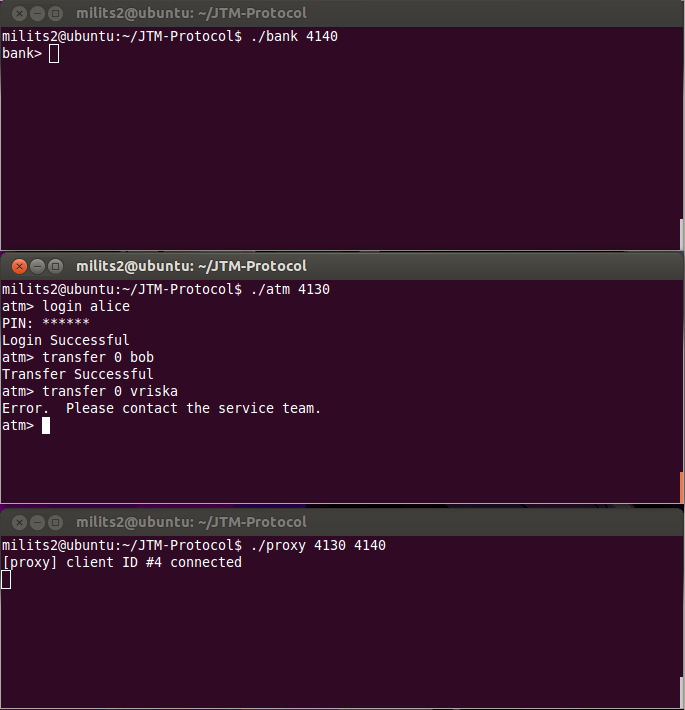
\includegraphics[scale=0.5]{transferUser.png}
\\

\section{Dysfunctional Card Verification}
The actual contents of a card file are ignored. The only verification done on the card is if it has anything in it. That is, any card put into the machine will satisfy it, as long as it doesn't have a blank "magnetic strip" (i.e., contents). This is a massive security flaw, as it is a failure of two-factor security. The only protection that ATMs have are PINs, which only have $10^6$ options.

\section{Poor Scaling}
While not an issue with the current scale of the project, all account information is stored in a vector. With O(n) lookups, this will become incredibly slow with very large amounts of users.

\section{Crashing the Bank}
Adding a single line of code to the proxy will crash the bank. The bank cannot handle a malformed handshake message. The follow section of code in the proxy:
\begin{lstlisting}
while(1)
{
	//read the packet from the ATM
    // [...]
	
	// Crashes bank
    strcpy( packet, "" );
    
	//forward packet to bank
    // [...]
	
	//get response packet from bank
    // [...]
	
	// Crashes ATM
	strcpy( packet, "" );
	
	//forward packet to ATM
    // [...]
}
\end{lstlisting}
can be easily manipulated to crash the bank (or, similarly, the ATMs, as detailed slightly later). Adding the line of code before forwarding the packet to the bank crashes the bank as soon as an ATM user attempts to log in. 
\\
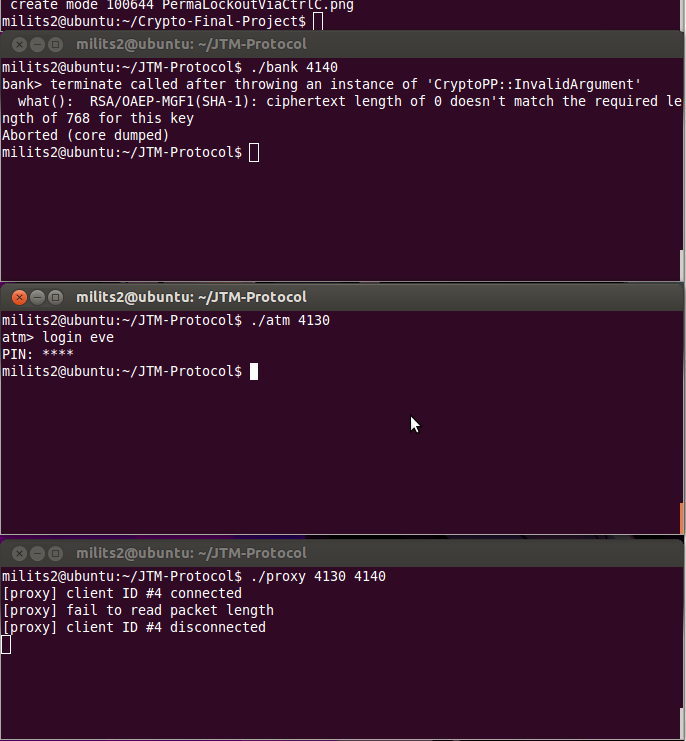
\includegraphics[scale=0.5]{crashBank.png}
\\
Similarly, ATMs can be crashed by adding the line of code before forwarding the packet to the ATM.
\\
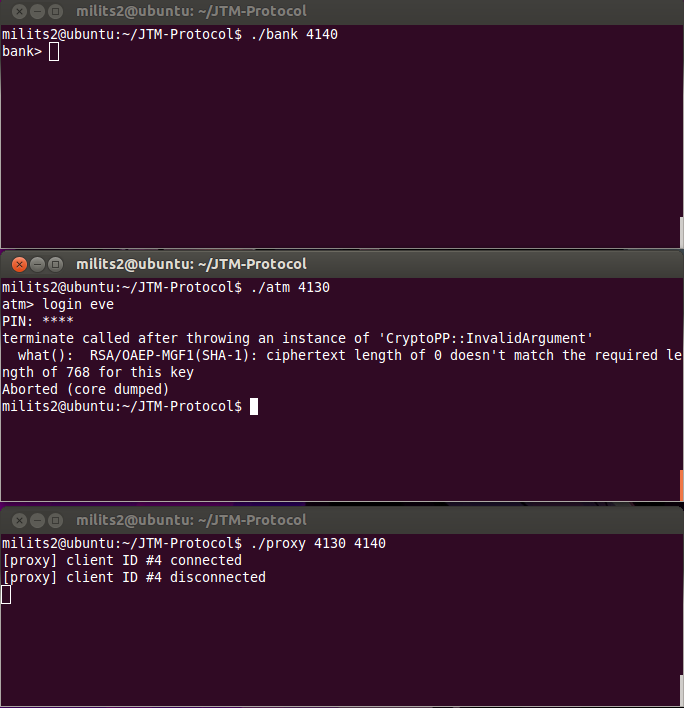
\includegraphics[scale=0.5]{crashATM.png}
\\
If both lines are left in, the bank crashes with a core dump, and the ATM crashes with no error message. This issue is due to not checking the validity of initial handshake messages. When it receives a blank message, it still tries to proceed with setting up a secure connection. The cryptographic functions crash, and the ATM and/or bank crash with them.

\section{RNG Flaws}

Their random number generator when asked for 32 bytes of data outputs 32
random hex bytes. This means that each byte only has 16 ($2^{4}$) possibilities instead
of 256 ($2^{8}$).

The end result is that everything generated using these functions (AES keys, nonces, etc.) only
have 128 bits of randomness instead of the expected 256 bits of randomness.

\begin{lstlisting}
std::string getRandom(int length)
{
     std::string retStr = "";
     CryptoPP::AutoSeededRandomPool rng;
     int random;
     int num = 0;
     bool hex = true;

     for(unsigned int i = 0; i < length; ++i)
     {
         random = (int) rng.GenerateByte();
         if(hex)
         {
             // Generate Random Hex String
             num = (int) (random % 16);
             if(num < 10)
             {
                 retStr += (num + '0');
             }
             else
             {
                 retStr += ((num - 10) + 'A');
             }
         }
         else
         {
             // Generate Random String With ASCII Range (48, 126)
             num = (int) (random % (126 - 48));
             retStr += (num + '0');
         }
     }

     return retStr;
}
\end{lstlisting}

\section{Login Info}

The login info is sent in cleartext inside of the encrypted packet.
By login info we mean the card number and pin.
The PIN is compared to the pin on the server. There is no hashing
of the login information.
The card number is not used.

\section{Handshake Hijacking}

When the bank and ATM establish a handshake the ATM sends the bank a 
nonce encrypted with the banks rsa key. Then the bank sends back an
encryption key and the nonce, as well as its own generated nonce.

Note that there is no explicit authentication.

Assuming you have the ATM's public key, it is possible to pretend to be the bank. You can simply send back a key encrypted with the ATM's public key and the nonce.

Since there is no RSA authentication, or any other form of authentication for that matter,
if you can guess the nonce you can masquerade as the bank. Normally this would
take $2^{256}$ attempts, but due to the aforementioned flaw in the RNG it only
takes $2^{128}$ attempts. Even worse, if you are starting an ATM on an embedded
system, upon restart the entropy will be low and it is possible to guess
the output of the system's random number generator. This makes pretending to be the bank even easier.

This is incredible useful due to the plethora of exploits available. You can 
make the ATM give out infinite money, and you can read everyone's card numbers 
and PINs since they are sent over the network unhashed.

\section{Key Management}

Their binary does not have keys hardcoded into it. Rather they must be put in a special folder. This has two issues. First it is much easier to make a copy of their keys
Second it allows for on the fly key manipulation. If you have access to the directory controlling the keys, you can change the keys and since the program loads them from disk each time it tries to use them you can change them at runtime.

\section{Bank Deposit Limits}
Due to the incorrect way atm limits are implemented, completely on the server side and globally, the bank is limited to depositing 1000\$ into any account. It cannot make multiple 1000\$ deposits.
\end{document}
